%% See: https://bookdown.org/yihui/rmarkdown-cookbook/multi-column.html
%% I've made some additional adjustments based on my own preferences (e.g. cols
%% should be top-aligned in case of uneven vertical length)
\newenvironment{columns}[1][]{}{}

\newenvironment{column}[1]{\begin{minipage}[t]{#1}\ignorespaces}{%
\end{minipage}
\ifhmode\unskip\fi
\aftergroup\useignorespacesandallpars
}

\def\useignorespacesandallpars#1\ignorespaces\fi{%
#1\fi\ignorespacesandallpars}

\makeatletter
\def\ignorespacesandallpars{%
  \@ifnextchar\par
    {\expandafter\ignorespacesandallpars\@gobble}%
    {}%
}
\makeatother


\title [Bootstrap]{ Cross Validation and Sample Splitting}
\author{C.Conlon}
\institute{Applied Econometrics II}
\date{\today}
\setbeamerfont{equation}{size=\tiny}
\begin{document}

\begin{frame}
\titlepage
\end{frame}



\begin{frame}{Cross Validation}
Cross Validation appears superficially similar to bootstrap but asks a different question.
\begin{itemize}
\item Bootstrap tries to construct an empirical analogue to the sampling distribution of $\hat{\theta}$.
\item CV tries to measure what the expected out of sample (OOS or EPE) prediction error of a new never seen before dataset.
\item The main consideration is to prevent \alert{overfitting}.
\begin{itemize}
\item In sample fit is always going to be maximized by the most complicated model.
\item OOS fit might be a different story.
\item 1-NN might do really well in-sample, but with a new sample might perform badly.
\end{itemize}
\end{itemize}
\end{frame}

\begin{frame}{Sample Splitting/Holdout Method and CV}
Cross Validation is actually a more complicated version of \alert{sample splitting} that is one of the organizing principles in machine learning literature.

\begin{description}
\item[Training Set] This is where you estimate parameter values.
\item[Validation Set] This is where you choose a model- a bandwidth $h$ or tuning parameter $\lambda$ by computing the error.
\item[Test Set] You are only allowed to look at this after you have chosen a model. \alert{Only Test Once}: compute the error again on fresh data.
\end{description}
\begin{itemize}
\item Conventional approach is to allocate 50-80\% to training and 10-20\% to Validation and Test.
\item Sometimes we don't have enough data to do this reliably.
\end{itemize}
\end{frame}

\begin{frame}{Sample Splitting/Holdout Method}
\begin{center}
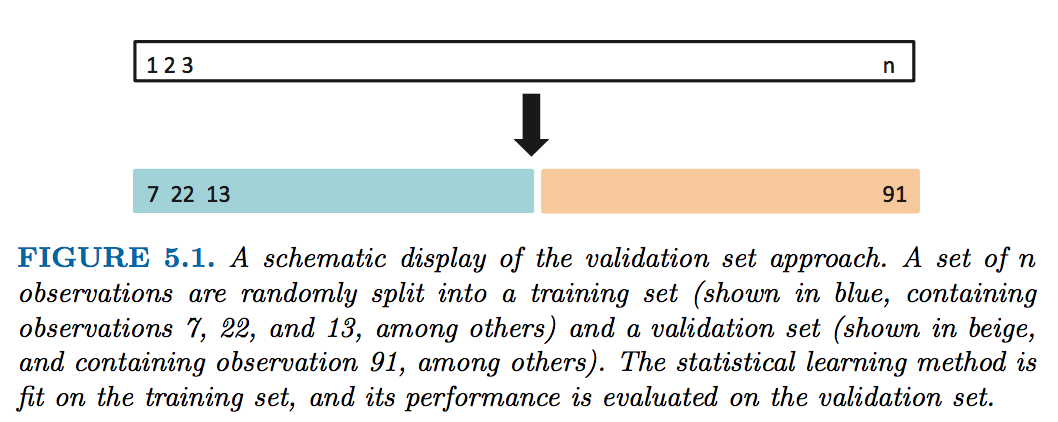
\includegraphics[width=4.5in]{./resources/split-sample}
\end{center}
\end{frame}

\begin{frame}{Challenge with Sample Splitting}
\begin{center}
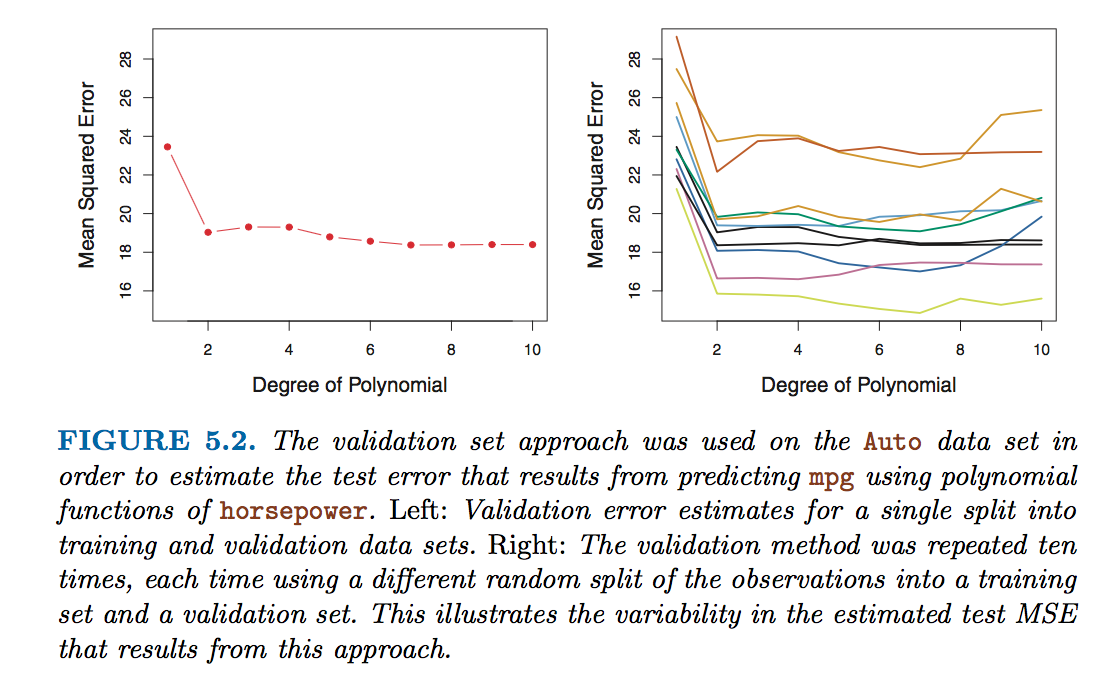
\includegraphics[width=4.5in]{./resources/validation-10fold}
\end{center}
\end{frame}


\begin{frame}{Cross Validation}
\begin{center}
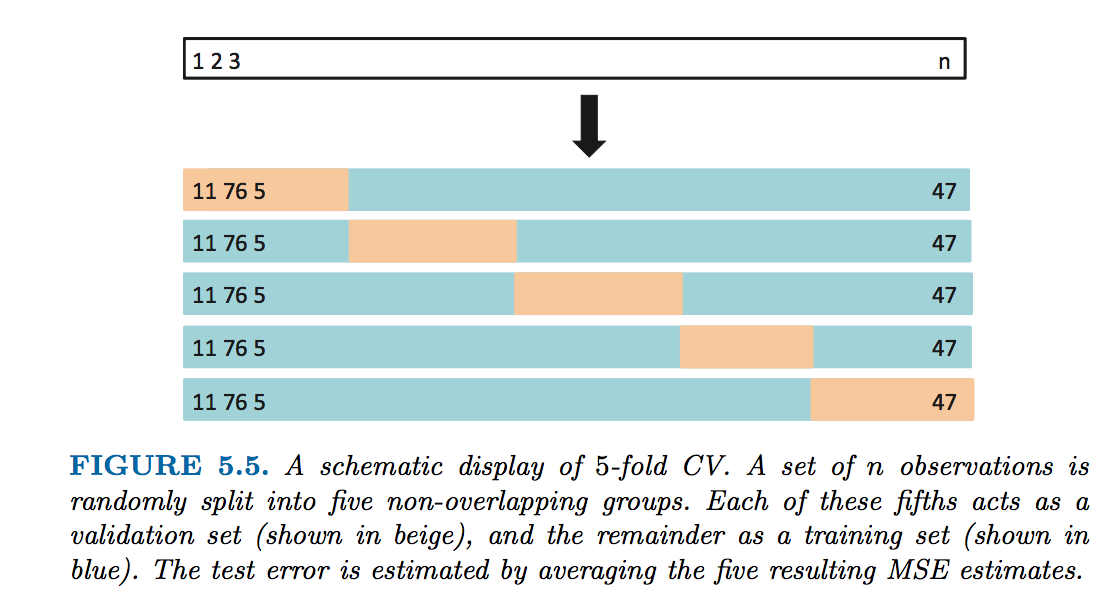
\includegraphics[width=4.5in]{./resources/split-cv5}
\end{center}
\end{frame}

\begin{frame}{$k$-fold Cross Validation}
\begin{itemize}
\item Break the dataset into $k$ equally sized ``folds'' (at random).
\item Withhold $i=1$ fold
\begin{itemize}
\item Estimate the model parameters $\hat{\theta}^{(-i)}$ on the remaining $k-1$ folds
\item Predict $\hat{y}^{(-i)}$ using $\hat{\theta}^{(-i)}$ estimates for the $i$th fold (withheld data).
\item Compute $MSE_i =\frac{1}{k \cdot N} \sum_j (y^{(-i)}_j -\hat{y}^{(-i)}_j)^2$.
\item Repeat for $i=1,\ldots,k$.
\end{itemize}
\item Construct $\widehat{MSE}_{k,CV} = \frac{1}{k} \sum_i MSE_{i}$
\end{itemize}
\end{frame}

\begin{frame}{Leave One Out Cross Validation (LOOCV)}
Same as $k$-fold but with $k=N$.
\begin{itemize}
\item Withhold a single observation $i$
\item Estimate $\hat{\theta}_{(-i)}$.
\item Predict $\hat{y}_i$ using $\hat{\theta}^{(-i)}$ estimates
\item Compute $MSE_i =\frac{1}{N} \sum_j (y_i -\hat{y}_i(\hat{\theta}^{(-i)}))^2$.
\end{itemize}
\vspace{0.2cm}
Note: this requires estimating the model $N$ times which can be costly.
\end{frame}



\begin{frame}{Cross Validation}
\begin{center}
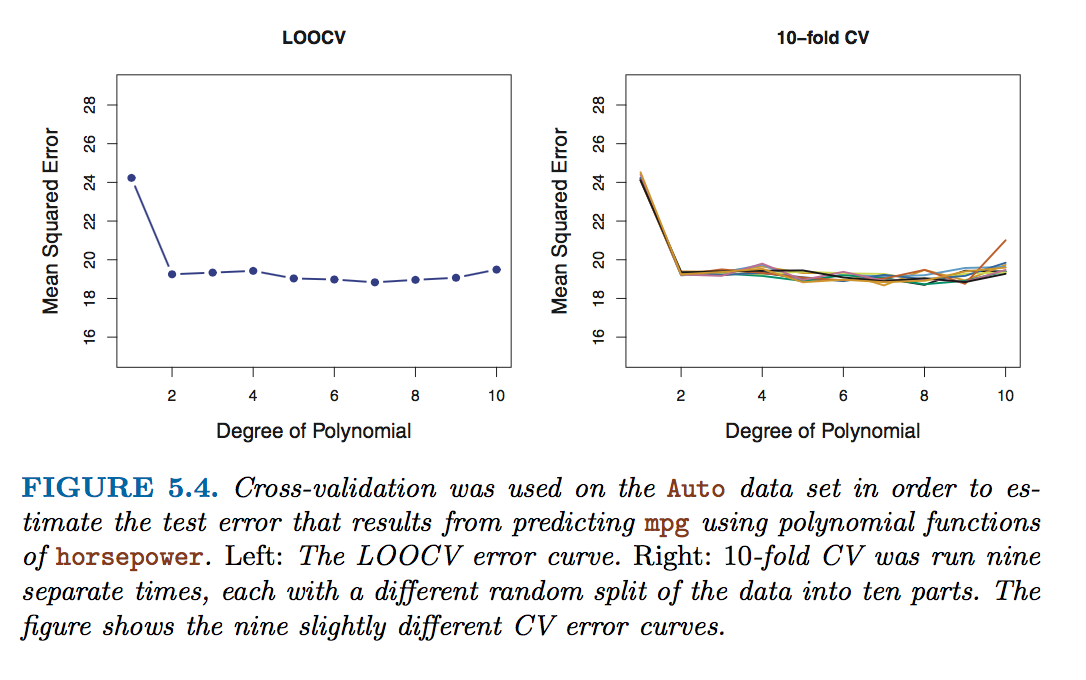
\includegraphics[width=4.5in]{./resources/comparison-cv}
\end{center}
\end{frame}

\begin{frame}{Cross Validation}
\begin{itemize}
\item Main advantage of cross validation is that we use all of the data in both \alert{estimation} and in \alert{validation}.
\begin{itemize}
\item For our purposes validation is mostly about choosing the right bandwidth or tuning parameter.
\end{itemize}
\item We have much lower variance in our estimate of the OOS mean squared error.
\begin{itemize}
\item Hopefully our bandwidth choice doesn't depend on randomness of splitting sample.
\end{itemize}
\end{itemize}
\end{frame}



\begin{frame}{Test Data}
\begin{itemize}
\item In Statistics/Machine learning there is a tradition to withhold 10\% of the data as \alert{Test Data}.
\item This is \alert{completely new data} that was not used in the CV procedure.
\item The idea is to report the results using this test data because it most accurately simulates true OOS performance.
\item We don't do much of this in economics.\\
 (Should we do more?)
\end{itemize}
\end{frame}





\end{document}